\documentclass
%[handout]
{beamer}
\documentclass{beamer}

%%
%%
%%
% From http://tex.stackexchange.com/questions/2072/beamer-navigation-circles-without-subsections
% Solution #2 or 3:
% \usepackage{etoolbox}
% \makeatletter
% % replace the subsection number test with a test that always returns true
% \patchcmd{\slideentry}{\ifnum#2>0}{\ifnum2>0}{}{\@error{unable to patch}}%
% \makeatother
% Solution #1:
\usepackage{remreset}% tiny package containing just the \@removefromreset command
\makeatletter
%\@removefromreset{subsection}{section}
%\makeatother
%\setcounter{subsection}{1}




\usepackage{etex}
\usepackage{pgf}
\usepackage{tikz}
\usepackage{url}
\usepackage{amsmath}
\usepackage{color}
% \definecolor{red}{rgb}{1,0,0}
\usepackage{ulem}
% \usepackage{booktabs}
\usepackage{colortbl,booktabs}
\renewcommand*{\thefootnote}{\fnsymbol{footnote}}
\usepackage{fancybox}
\usepackage[framemethod=TikZ]{mdframed}
\mdfdefinestyle{FactStyle}{%
  outerlinewidth=0.5,
  roundcorner=1pt,
  leftmargin=1cm,
  linecolor=blue,
  outerlinecolor=blue!70!black,
  backgroundcolor=yellow!40
}
\usepackage{cancel}

  \newcommand\Warning{%
    \makebox[2.4em][c]{%
      \makebox[0pt][c]{\raisebox{.2em}{\Large!}}%
      \makebox[0pt][c]{\color{red}\Huge$\bigtriangleup$}}}%

\usepackage{stackengine}
\usepackage{scalerel}
\usepackage{xcolor}
  \newcommand\dangersign[1][2ex]{%
    \renewcommand\stacktype{L}%
    \scaleto{\stackon[1.3pt]{\color{red}$\triangle$}{\tiny !}}{#1}%
  }



\usepackage{dcolumn}
\newcolumntype{d}[1]{D{.}{.}{#1}}

% From
% http://tex.stackexchange.com/questions/109900/how-can-i-box-multiple-aligned-equations
\usepackage{empheq}
\usepackage{tcolorbox}  \newtcbox{\othermathbox}[1][]{%
  nobeforeafter, tcbox raise base, 
  colback=black!10, colframe=red!30, 
  left=1em, top=0.5em, right=1em, bottom=0.5em}

\newcommand\blue{\color{blue}}
\newcommand\red{\color{red}}
\newcommand\green{\color{green!75!black}}
\newcommand\purple{\color{purple}}
\newcommand\bluegreen{\color{blue!75!green}}
\newcommand\orange{\color{orange}}
\newcommand\redgreen{\color{red!50!green}}
\newcommand\grey{\color{black}}
\newcommand\gap{\vspace{.1in}}
\newcommand\nb{${\red\bullet}\ $}
\newcommand\halfgap{\vspace{.05in}}
\newcommand\divideline{\line(1,0){352}}
\usepackage{marvosym} % for \Smiley

\newcommand{\bluealert}[1]{{\blue\textbf{#1}}}

% \usepackage{beamerthemesplit} %Key package for beamer
\usetheme{Singapore}
% \usetheme{Szeged}
% \usetheme{Garfield}
% \usetheme{CambridgeUS}
% \usenavigationsymbolstemplate{} %Gets rid of slide navigation symbols


\setbeamercolor{separation line}{use=structure,bg=structure.fg!50!bg}
% \begin{beamercolorbox}[colsep=0.5pt]
%   {upper separation line foot}
% \end{beamercolorbox}



\makeatletter
\setbeamertemplate{footline}
{
  \leavevmode%
  \hbox{%
% \begin{beamercolorbox}[colsep=0.5pt]
%   {upper separation line foot}
% \end{beamercolorbox}


  \begin{beamercolorbox}[wd=.5\paperwidth,ht=2.25ex,dp=2ex,colsep=0.5pt]%
    {upper separation line foot}
    \usebeamerfont{author in head/foot}%
    \hspace*{2ex}\insertshortdate:\ \insertshorttitle
  \end{beamercolorbox}%
  \begin{beamercolorbox}[wd=.5\paperwidth,ht=2.25ex,dp=2ex,right]{title in head/foot}%
    \usebeamerfont{title in head/foot}
    {\insertshortauthor}\hspace*{2ex}
  \end{beamercolorbox}}%
  % \begin{beamercolorbox}[wd=.333333\paperwidth,ht=2.25ex,dp=2ex,right]{date in head/foot}%
  %   \usebeamerfont{date in head/foot}\insertshortdate{}\hspace*{2em}
  %   \insertframenumber{} / \inserttotalframenumber\hspace*{2ex} 
  % \end{beamercolorbox}%
  \vskip0pt%
}
\makeatother

\usetikzlibrary{decorations.markings}
\usetikzlibrary{arrows}


\title{Final Exam Review}
\author{Schley, UCSB Mathematics}
\date{March 15, 2017}
%\institute{}


\useinnertheme{default}

\usefonttheme{serif}
% \usecolortheme{rose}
% \usecolortheme{whale}
% \usecolortheme{orchid}
\usecolortheme{crane}
% \usecolortheme{dolphin}


%TEMPLATE
\setbeamertemplate{navigation symbols}{}

\setbeamertemplate{note page}[compress]

\setbeamertemplate{frametitle}{
  \vspace{0.5em}
  % \begin{centering}
  {\huge\blue\textbf{\textmd{\insertframetitle}}}
  \par
  % \end{centering}
}

% From http://tex.stackexchange.com/questions/7032/good-way-to-make-textcircled-numbers:
\newcommand*\circled[1]{\tikz[baseline=(char.base)]{\node[shape=circle,draw,fill=orange,inner sep=1pt] (char) {#1};}} 
% \renewcommand{\labelenumi}{\circled{\textbf{\arabic{enumi}}}}

\let\olddescription\description
\let\oldenddescription\enddescription
\usepackage{enumitem}
\let\description\olddescription
\let\enddescription\oldenddescription

% \usepackage[loadonly]{enumitem}
\setlist[enumerate,1]{label=\colorbox{orange}{\arabic*.},font=\bfseries}
%\setlist[enumerate,2]{label=\colorbox{blue!25}{(\alph*)},font=\bfseries}
% \setlist[enumerate,1]{label=\arabic*.,font=\bfseries}
\setlist[itemize,1]{label=\red$\bullet$}
\setlist[itemize,2]{label=\blue$\bullet$}

\newcommand\answer[1]{\fbox{#1}}
% \renewcommand\answer[1]{}

\newcommand{\antilog}{\operatorname{antilog}}

\newcommand{\instructor}{Nathan Schley ({\it Sh}+{\it lye})}
\newcommand{\officehours}{T R 11-11:50, T 3:45-4:35 Details on Gauchospace.}
\newcommand{\email}{schley@math.ucsb.edu}
\newcommand{\officeloc}{South Hall 6701}
\newcommand{\copyrightinfo}{2022\ Daryl Cooper, Peter M.\ Garfield, Ebrahim Ebrahim \& Nathan Schley}
    














\title{}
\title{Calculus Intro}
\date{May 12, 2022}


\begin{document}
\small



\section*{Administration}

\frame{
  \frametitle{}
  {\Huge{}Welcome Back!}\\[.5em]

  {\Huge{}Differential Calculus}
  \vfill
  {\Large{}Instructor:}\\
  \ \hspace*{0.2in} Nathan Schley ({\it Sh}+{\it lye}), \url{schley@math.ucsb.edu}\\
  \ \hspace*{0.2in} South Hall 6701
  \\[0.5em]

  {\Large{}Office Hours:}\\
  \ \hspace*{0.2in} T R 11-11:50, T 3:45-4:35 Details on Gauchospace. 
  \bigskip

  \copyright\ 2022\ Daryl Cooper, Peter M.\ Garfield, Ebrahim Ebrahim \& Nathan Schley\\
  Please do not distribute outside of this course.
  \vfill

}


\section{Linear Approximations}


\frame{
Suppose $x$ and $y$ are related variables. So as one changes, the other changes.
We can ask:
\begin{center}
\textit{How much does $y$ change per unit change in $x$?}
\end{center}
Answer: The derivative of $y$ with respect to $x$ tells us, and it depends on the current value of $x$! 

\vspace{1em}

If we write $y$ as a function of $x$ like this: $y=f(x)$, then the derivative is written as
$$
\begin{array}{ccccc}
\dfrac{\textrm{d}y}{\textrm{d}x} & \text{or} & \dfrac{\textrm{d}f}{\textrm{d}x} & \text{or} & f'(x)
\end{array}
$$
It is the limit of ``average rate of change'' over shorter and shorter $\Delta x$:
$$ f'(x) = \lim_{h \rightarrow 0} \frac{f(x+h)-f(x)}{h} $$
also known as ``instantaneous rate of change''
}


\frame{
 \frametitle{Why use $h$ to find the derivative?}
   {\large\blue$$\text{Without $h$: \ }\fbox{f'(x) = \lim_{\chi \rightarrow x} \frac{f(\chi)-f(x)}{\chi-x}}$$}
   Here is an example without $h$. For $f(x) = x^2$, if we wanted to find $f'(2)$ it would be the limit of the average rate of change from 2 to a second point $\chi$ as that second point approaches 2. \pause
   $$\underset{\chi\rightarrow2}{\lim} \frac{\chi^2 - 2^2}{\chi-2}\pause=\underset{\chi\rightarrow2}{\lim} \frac{(\chi - 2)(\chi+2)}{(\chi-2)}\pause=\underset{\chi\rightarrow2}{\lim} \ \chi + 2\pause=4$$\pause
   Second example: For $g(x) = x^3$, if we wanted to find $g'(5)$ it would be the limit of the average rate of change from 5 to a second point $\chi$ as that second point approaches 5. \pause
   $$\underset{\chi\rightarrow5}{\lim} \frac{\chi^3 - 5^3}{\chi-5}\pause=\underset{\chi\rightarrow5}{\lim} \frac{(\chi - 5)(\chi^2+5\chi + 5^2)}{(\chi-5)}\pause=\underset{\chi\rightarrow5}{\lim} \ \chi^2+5\chi + 5^2\pause=75$$ \pause
   {\large\blue It's often harder to find the derivative this way, so we just make $\Delta x = h$ and let $h$ disappear.}
   
   
   
}


\frame{
 \frametitle{On the other hand...}
   {\large\blue$$\text{With $h$: \ }\fbox{f'(x) = \lim_{h \rightarrow 0} \frac{f(x+h)-f(x)}{h}}$$}
   For $f(x) = x^2$, we can find $f'(2)$ this way. \pause
   $$\underset{h\rightarrow0}{\lim} \frac{(2+h)^2 - 2^2}{h}\pause=\underset{h\rightarrow0}{\lim} \frac{2^2 + 4h + h^2 - 2^2}{h}\pause=\underset{h\rightarrow0}{\lim} \frac{4h + h^2}{h}\pause$$
   $$=\underset{h\rightarrow0}{\lim} \ 4 + h\pause=4$$\pause
   For $g(x) = x^3$, we can find $g'(5)$ this way. \pause
   $$\underset{h\rightarrow0}{\lim} \frac{(5+h)^3 - 5^3}{h}\pause=\underset{h\rightarrow0}{\lim} \frac{5^3 + 75h + 15h^2 + h^3 - 5^3}{h}\pause=\underset{h\rightarrow0}{\lim} \frac{75h + 15h^2 + h^3}{h}\pause$$
   $$=\underset{h\rightarrow0}{\lim} \ 75 + 15h + h^2\pause=75$$\pause
   {\large\blue What do you think?} \pause \\ \fbox{A} $h$ is easier! \ \fbox{B} Nah, difference of cubes ftw! \\
   \phantom{.}
   
   
   
}


\frame{
  \frametitle{\S8.6: Tangent Line Approximation}

  \alert{Question:}\ At 5am the temperature is $42^{\circ}\ \text{F}$ and increasing
  at a rate of $10^{\circ}\ \text{F}$ per hour. Which of the following do you think
  is closest to the temperature at 5:15am? 
  \begin{center}
    A$ = 2.5^{\circ}\ \text{F}$
    \quad 
    B$ = 52^{\circ}\ \text{F}$
    \quad 
    C$ = 43.5^{\circ}\ \text{F}$
    \quad 
    D$ = 44.5^{\circ}\ \text{F}$
    \quad 
    E$ =5.15^{\circ}\ \text{F}$
  \end{center}
  \pause
  \alert{Answer:}\ 
    \fbox{D}

    % \gap  5:15 is $1/4$ of an hour after 5am.\\
    % $\therefore\quad$ Temperature rises {\blue approximately} $(1/4)\times 10=2.5^{\circ}\ \text{F}$ in this time.\\
    % So final temperature is {\blue approximately} $42+2.5=44.5^{\circ}\ \text{F}.$

    % \gap
    % {\blue Approximately} because instantaneous rate of change is $10$ at $5am$ but this may change. Maybe by 5:10am temperature is increasing at a rate of $11^{\circ}\ \text{F}$ per hour.

    % \gap
    % Answer is \fbox{{\blue (initial temperature)} + {\red (rise in temperature)}}\\
    % {\red (rise in temperature)} $\approx$ (time taken) $\times$ {\green (rate of change)}
    
    % {\green rate of change} = {\green derivative}

    % \gap 
    % \includegraphics[scale=0.6]{inputoutput.pdf}

    \begin{center}
      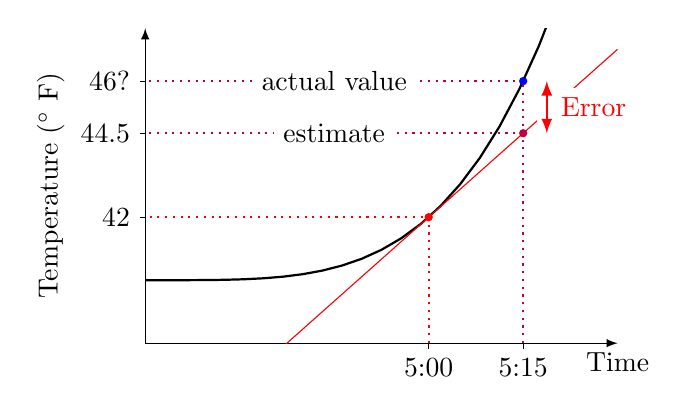
\begin{tikzpicture}[x=12mm,y=8mm,>=latex]
        \draw[thin,black,->] (0,0) -- (5,0) node[below] {Time};
        \draw[thin,black,->] (0,0) -- (0,5);
        \node[rotate=90] at (-1,2.5) {Temperature (${}^\circ\ \text{F}$)};
        \begin{scope}
          \clip (0,0) rectangle (5,5);
          \draw[thick,black,domain=0:5] plot (\x,{1+(\x/3)^4});
          % tangent line at (3,2) is y-2=(4/3)(x-3) or y=4x/3-2:
          \draw[thin,red,domain=0:5] plot (\x,{4*\x/3-2});
        \end{scope}
        \draw[black,thin] (3,0) -- (3,-2pt) node[below] {5:00};
        \draw[black,thin] (4,0) -- (4,-2pt) node[below] {5:15};
        \draw[black,thin] (0,2) -- (-2pt,2) node[left] {$42$};
        \draw[red,thick,dotted] (3,0) -- (3,2) -- (0,2);
        \fill[red] (3,2) circle (1.5pt);
        \fill[purple] (4,{4*4/3-2}) circle (1.5pt);
        \draw[thick,dotted,purple] (4,0) -- (4,{1+(4/3)^4});
        \draw[thick,dotted,purple] (4,{4*4/3-2}) -- (0,{4*4/3-2}) node[midway,black,fill=white] {estimate};
        \draw[black,thin] (0,{4*4/3-2}) -- (-2pt,{4*4/3-2}) node[left] {$44.5$};
        \draw[thick,dotted,purple] (4,{1+(4/3)^4}) -- (0,{1+(4/3)^4}) node[midway,black,fill=white] {actual value};
        \draw[black,thin] (0,{1+(4/3)^4}) -- (-2pt,{1+(4/3)^4}) node[left] {$46$?};
        \fill[blue] (4,{1+(4/3)^4}) circle (1.5pt);
        \filldraw[white] (4.15,{4*4/3-2-0.5}) rectangle (4.5,{1+(4/3)^4+0.25});
        \draw[red,thick,fill=white,<->] (4.25,{4*4/3-2}) -- (4.25,{1+(4/3)^4}) node[midway,right,red,fill=white,xshift=0.5mm] {Error};
      \end{tikzpicture}
    \end{center}
  
}



\frame{
  \frametitle{Continuing this example}
  
  Same set-up:
  \begin{itemize}
  \item $f({\red x})=$ temperature at {\red time $x$}\ hours after midnight

  \item $f(5)=42$ ($42^{\circ}\ \text{F}$ at 5:00am)

  \item $f{\red'}(5)=2$
  \end{itemize}

  \alert{(1)}\ Find the equation of {\blue tangent line} to $y=f(x)$ at $x=5$.

  \begin{center}
    A\ \ $y = 5x+42$
    \qquad
    B\ \ $y = 2x+5$
    \qquad
    C\ \ $y = 2(x-5)+42$
    \\
    D \ \  $y -5 = 2(x-42)$ 
    \qquad
    E \ \  $y -42 = 2x-5$ 
  \end{center}
  \pause
  \alert{Answer:}\ \fbox{C}
  \pause

  \alert{(2)}\ Use this to predict the approximate temperature at 4am.
  \begin{center}
    A$ = 40$
    \quad 
    B$ = 41$
    \quad 
    C$ = 42$
    \quad 
    D$ = 43$
    \quad 
    E$ = 44$
    \pause
    \quad
    \fbox{A}
  \end{center}
  \pause

  \alert{(3)}\ The tangent line approximation is used to estimate the
  temperature at the following times. Which do you think is most
  accurate?
  \begin{center}
    A\ 4am
    \quad 
    B\ 4:50am
    \quad 
    C\ 5:25am
    \quad 
    D\ 6am
    \quad 
    E\ midnight
    \quad
    \pause
    \fbox{B}
  \end{center}

}


\frame{
  \frametitle{Tangent Line Approximation}

  To do a tangent line approximation:
  \begin{itemize}
  \item[(i)] Find the equation of the tangent line.

  \item[(ii)] Plug in the required value(s) into this equation.

  \end{itemize}
  \gap

  Suppose $f({\orange 4})={\blue 2}$ and $f{\red'}({\orange 4})={\red 3}$.

  \begin{itemize}
  \item[\red(a)]  The equation of the tangent line to $y=f(x)$ at $x={\orange 4}$ is $y=$?
    \begin{center}
      A$ = {\orange 4}x-{\purple 14}$
      \qquad 
      B$= {\orange 3}x-{\purple 10}$
      \qquad 
      C$= {\orange 2}x-{\purple 6}$
      \\
      \ \hfill
      D$={\orange 3}x-{\purple 4}$
      \qquad 
      E$= {\orange 2}x-{\purple 5}$
      \pause 
      \hfill
      \fbox{B}
    \end{center}
    \pause

  \item[\red(b)] Use this tangent line approximation to estimate $f(4.1)$.
    \begin{center}
      A$=2.3$
      \quad 
      B$= 1.7$
      \quad 
      C$ = 2.6$
      \quad 
      D$ = 1.4$
      \quad 
      E$ = 2$
      \pause
      \quad
      \fbox{A}
    \end{center}


  \item[\red(c)]
    Use the tangent line approximation to estimate the value of $x$ which gives $f(x)=2.9$.
    \begin{center}
      A$ = 4.9$
      \quad 
      B$ = 4.1$
      \quad 
      C$ = 2.9$
      \quad 
      D$ = 4.1$
      \quad 
      E$ = 4.3$
      \pause
      \quad
      \fbox{E}
    \end{center}
  \end{itemize}

}

\frame{
  \frametitle{Standard Estimation Problem}

  \alert{Question:}\ Approximate $\sqrt{26}$.

  \begin{center}
    A$=0.1$
    \quad 
    B$= 5.01$
    \quad 
    C$ = 5.05$
    \quad 
    D$ = 5.1$
    \quad 
    E$ = 5.2$
    \quad
    \uncover<3->{\fbox{D}}
  \end{center}

  \uncover<2->{%
    \alert{Some tools:}\ For $g(x)=\sqrt{x}$, $g{\red'}({\blue 25})={\red
      1/10}$ and $g({\blue25}) = \sqrt{\blue 25}={\bluegreen 5}$.
  }
  \gap
  \gap

  \uncover<4->{%
    \alert{Better estimate:}\ $\sqrt{26}\approx5.09902$, so the {\red
      error} in the tangent line approximation here is
    \begin{equation*}
      \text{\red{}error} 
      \approx 5.1-5.09902
      \approx0.001
    \end{equation*}
    This is a percentage error of only $\red 0.02\%$.
  }

}


\frame{
  \frametitle{Another Example:}

  \begin{itemize}
  \item $f(t) = \text{number of grams of a chemical reagent after $t$
      seconds}$
    \smallskip

  \item We're told $f(0)=20$ and $f{\red'}(0)=-3$
    \smallskip
  \end{itemize}

  \alert{Question:}\ Roughly how many grams are there after $t$ seconds?

  \begin{center}
    A$=4-3t$
    \quad 
    B$= 20-3t$
    \quad 
    C$ = 20-4t$
    \quad 
    D$ =20 + 4t$
    \quad 
    E$ = 32-3t$
  \end{center}
  \pause

  \alert{Answer:}\ \fbox{B}


}





\section{Sketching Curves}

\frame{
  \frametitle{Sketching some simple graphs}

  It's useful to be able to sketch\ldots
  \smallskip

  \alert{(1)\ Quadratics}

  \begin{minipage}{0.45\linewidth}
    \begin{center}
      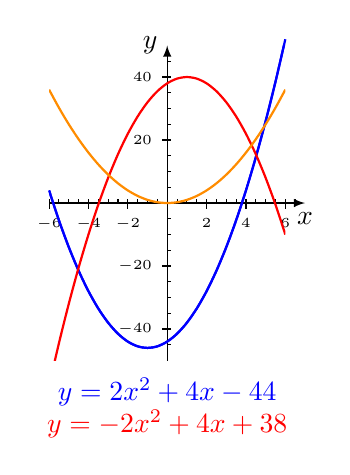
\begin{tikzpicture}[x=2.5mm,y=0.4mm,>=latex]
        \draw[thin,black,->] (-6,0) -- (7,0) node[below] {$x$};
        \draw[thin,black,->] (0,-50) -- (0,50) node[left] {$y$};
        % ticks:
        \foreach \x in {-6,-4,-2,2,4,6}
        {
          \draw[thin,black] (\x,0) -- (\x,-2pt) node[below] {$\scriptscriptstyle\x$};
        }
        \foreach \x in {-6,-5.5,...,6.5}
        {
          \draw[thin,black] (\x,0) -- (\x,1.5pt);
        }
        \foreach \y in {-40,-20,20,40}
        {
          \draw[thin,black] (0,\y) -- (-2pt,\y) node[left] {$\scriptscriptstyle\y$};
        }
        \foreach \y in {-45,-40,...,45}
        {
          \draw[thin,black] (0,\y) -- (1.5pt,\y);
        }
        \draw[thick,blue,domain=-6:6,smooth] plot (\x,{2*(\x)^2+4*\x-44});
        % graphs:
        \begin{scope}
          \clip (-6,-50) rectangle (6,50);
          \draw[thick,blue,domain=-6:6,smooth] plot (\x,{2*(\x)^2+4*\x-44});
          \draw[thick,red,domain=-6:6,smooth] plot (\x,{-2*(\x)^2+4*\x+38});
          \uncover<2->{%
            \draw[thick,orange!90!yellow,domain=-6:6,smooth] plot (\x,{(\x)^2});
          }
        \end{scope}
        % labels:
        \node[blue] at (0,-60) {$y=2x^2+4x-44$};
        \node[red] at (0,-70) {$y=-2x^2+4x+38$};
      \end{tikzpicture}
    \end{center}
  \end{minipage}
  \hfill
  \begin{minipage}{0.5\linewidth}
    \begin{itemize}
    \item $y=ax^2+bx+c$
    \item Bowl-shaped:
      \begin{itemize}
      \item[\red$\star$] Opens up if $a>0$
      \item[\red$\star$] Opens down if $a<0$
      \end{itemize}
    \item Model curve: $y=x^2$ \\
      \uncover<2->{\colorbox{blue!25}{\color{orange!90!yellow}Shown here!}}
    \end{itemize}
  \end{minipage}
  \vspace*{2in}

}

\frame{
  \frametitle{Sketching some simple graphs}


  It's useful to be able to sketch\ldots
  \smallskip

  \alert{(2)\ Cubics}

  \begin{minipage}{0.45\linewidth}
    \begin{center}
      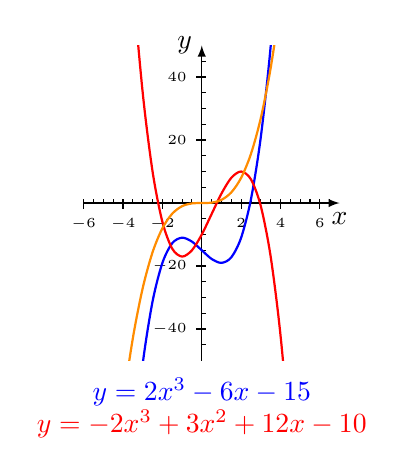
\begin{tikzpicture}[x=2.5mm,y=0.4mm,>=latex]
        \draw[thin,black,->] (-6,0) -- (7,0) node[below] {$x$};
        \draw[thin,black,->] (0,-50) -- (0,50) node[left] {$y$};
        % ticks:
        \foreach \x in {-6,-4,-2,2,4,6}
        {
          \draw[thin,black] (\x,0) -- (\x,-2pt) node[below] {$\scriptscriptstyle\x$};
        }
        \foreach \x in {-6,-5.5,...,6.5}
        {
          \draw[thin,black] (\x,0) -- (\x,1.5pt);
        }
        \foreach \y in {-40,-20,20,40}
        {
          \draw[thin,black] (0,\y) -- (-2pt,\y) node[left] {$\scriptscriptstyle\y$};
        }
        \foreach \y in {-45,-40,...,45}
        {
          \draw[thin,black] (0,\y) -- (1.5pt,\y);
        }
        % graphs:
        \begin{scope}
          \clip (-6,-50) rectangle (6,50);
          \draw[thick,blue,domain=-6:6,smooth] plot (\x,{2*(\x)^3-6*\x-15});
          \draw[thick,red,domain=-6:6,smooth] plot (\x,{-2*(\x)^3+3*(\x)^2+12*\x-10});
          \uncover<2->{%
            \draw[thick,orange!90!yellow,domain=-6:6,smooth] plot (\x,{(\x)^3});
          }
        \end{scope}
        % labels:
        \node[blue] at (0,-60) {$y=2x^3-6x-15$};
        \node[red] at (0,-70) {$y=-2x^3+3x^2+12x-10$};
      \end{tikzpicture}
    \end{center}
  \end{minipage}
  \hfill
  \begin{minipage}{0.5\linewidth}
    \begin{itemize}
    \item $y=ax^3+bx^2+cx+d$
    \item ``S''-shaped:
      \begin{itemize}
      \item[\red$\star$] Goes to $+\infty$ if $a>0$
      \item[\red$\star$] Goes to $-\infty$ if $a<0$
      \end{itemize}
    \item Model curve: $y=x^3$ \\
      \uncover<2->{\colorbox{blue!25}{\color{orange!90!yellow}Shown here!}}
    \end{itemize}
  \end{minipage}
  \smallskip
  \uncover<3->{%
    \begin{empheq}[box=\othermathbox]{align*}
      \text{For a polynomial, the {\blue highest power}\ of $x$ {\red dominates}\ when $x$ is big}    
    \end{empheq}
  }
  \vspace*{2in}



}

\section{Computing Derivatives}

\frame{
  \frametitle{The Derivatives of Simple Functions}

  \begin{minipage}{0.45\linewidth}
    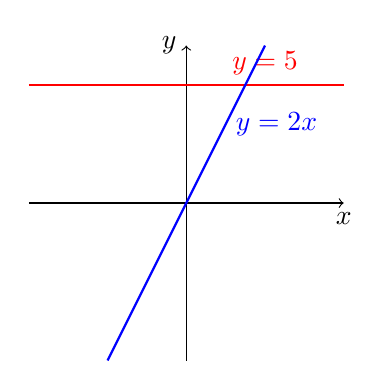
\begin{tikzpicture}
      \draw[thin,black,->] (-2,0) -- (2,0) node[below] {$x$};
      \draw[thin,black,->] (0,-2) -- (0,2) node[left] {$y$};
      \uncover<1-4>{%
        \draw[thick,red] (-2,1.5) -- (2,1.5) node[near end,above] {$y=5$};
      }
      \uncover<5->{%
        \draw[thick,blue] (-1,-2) -- (1,2) node[near end,right] {$y=2x$};
      }
    \end{tikzpicture}
  \end{minipage}
  \hfill
  \begin{minipage}{0.52\linewidth}
    The derivative of a constant is\only<1>{\ldots?}%
    \uncover<2->{%
      \ zero because:
       \begin{itemize}
       \item {\red$\text{derivative} = \text{rate of change}$}
       \item {\red constants don't change}\\[0.5em]
         \uncover<3->{%
       \item {\blue$\text{derivative} = \text{slope}$}
       \item {\blue$\text{slope} = 0$}
         }
       \end{itemize}
      \uncover<4->{So $\dfrac{d}{dx} \big( 5 \big) = 0$}
     }
  \end{minipage}
  \medskip

  \uncover<5->{%
    The derivative of a straight line is\only<5>{\ldots?}}\only<6->{%
    \ its slope because}
  \uncover<6->{%
    \begin{itemize}
    \item {\blue$\text{derivative} = \text{slope}$}
    \end{itemize}
  }
  \uncover<7->{So $\dfrac{d}{dx}\big(2x\big) = 2$}

}


\frame{
  \frametitle{Meaning of Derivatives}

  \begin{minipage}{0.45\linewidth}
    \begin{empheq}[box=\othermathbox]{align*}
      \Large%
      \frac{d}{dx}\left( x^2\right) = 2x      
    \end{empheq}
    % \vspace{.1in}

    What this {\blue means}
    %% \vspace{.1in}

    \begin{empheq}[box=\othermathbox]{align*}
      \text{The {\red slope} of the graph\ }\\
      \text{of ${\blue y=x^2}$ at $x={\red a}$ is $2{\red a}$}
    \end{empheq}
  \end{minipage}
  \hspace*{0.25in}
  \begin{minipage}{0.45\linewidth}
    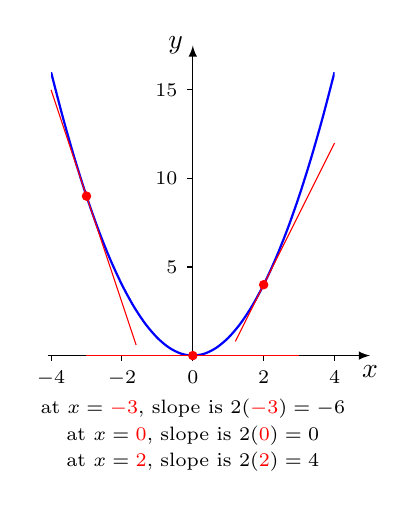
\begin{tikzpicture}[x=4.5mm,y=2.25mm,>=latex]
      \draw[thin,black,->] (-4.1,0) -- (5,0) node[below] {$x$};
      \draw[thin,black,->] (0,0) -- (0,17.5) node[left] {$y$};
      % ticks:
      \foreach \x in {-4,-2,0,2,4}
      {
        \draw[thin,black] (\x,0) -- (\x,-2pt) node[below] {$\scriptstyle\x$};
      }
      \foreach \y in {5,10,15}
      {
        \draw[thin,black] (0,\y) -- (-2pt,\y) node[left] {$\scriptstyle\y$};
      }
      \begin{scope}
        \clip (-4,0) rectangle (4,16);
        \draw[blue,thick,domain=-4:4,smooth] plot (\x,{(\x)^2});
      \end{scope}
      \uncover<2>{%
        \node at (0,-3) {$\scriptstyle\text{at $x={\red-3}$, slope is $2({\red-3})=-6$}$};
        % tangent line is y-9=-6(x+3) or y=-6x-9
        \draw[thin,red,domain=-4:-1.6] plot (\x,{-6*\x - 9});
        \filldraw[red] (-3,9) circle (1.5pt);
      };
      \uncover<3>{%
        \node at (0,-4.5) {$\scriptstyle\text{at $x={\red0}$, slope is $2({\red0})=0$}$};
        % tangent line is y=0
        \draw[thin,red] (-3,0) -- (3,0);
        \filldraw[red] (0,0) circle (1.5pt);
      };
      \uncover<4->{%
        \node at (0,-6) {$\scriptstyle\text{at $x={\red2}$, slope is $2({\red2})=4$}$};
        % tangent line is y-4=4(x-2) or y=4x-4
        \draw[thin,red,domain=1.2:4] plot (\x,{4*\x - 4});
        \filldraw[red] (2,4) circle (1.5pt);
      };
    \end{tikzpicture}
  \end{minipage}
  % \gap

  \uncover<5->{%
    \begin{empheq}[box=\othermathbox]{align*}
      \text{derivative}
      = \text{rate of change}
      = \text{slope of graph}
      = \text{slope of tangent line}
    \end{empheq}
  }



}



\frame{
  \frametitle{General Rule:}

  \begin{minipage}{0.45\linewidth}
    \begin{align*}
      \frac{d}{dx}\left(x^{\red 2}\right) & = {\red 2}x\\
      \frac{d}{dx}\left(x^{\red 3}\right) & = {\red 3}x^{\blue 2}\\
      \frac{d}{dx}\left(x^{\red 4}\right) & = {\red 4}x^{\blue 3}
    \end{align*}
  \end{minipage}
  \begin{minipage}{0.45\linewidth}
    \uncover<2->{%
      \begin{empheq}[box=\othermathbox]{align*}
        \frac{d}{dx}\left(x^{\red n}\right) & = {\red n}x^{\blue n-1}
      \end{empheq}
    }
  \end{minipage}
  \smallskip
  
  \uncover<3->{%
    The {\red exponent} comes out front. Then {\blue subtract} one
    from exponent.
  }

  \uncover<4->{\alert{Examples:}}
  \pause\pause\pause\pause

  \begin{enumerate}
  \item $\dfrac{d}{dx}\left( x^{\red 7}\right) = $
    \begin{center}
      A$ = 7x^7$
      \quad 
      B$ = 6x^6$
      \quad 
      C$ = 6x^7$
      \quad 
      D$ = 7x^6$
      \quad 
      E$ = 0$
      \quad
      \pause
      \answer{D}
    \end{center}

    \item $\dfrac{d}{dx}\left( x^{\red -3}\right) = $
      \begin{center}
        A$ = 3x^{-2}$
        \quad 
        B$ = -3x^{-2}$
        \quad 
        C$ = -2x^{-4}$
        \quad 
        D$ = -3x^{-4}$
        \quad
        \pause
        \answer{D}
      \end{center}

    \end{enumerate}

}

\frame{
  \frametitle{More Examples}
  \begin{empheq}[box=\othermathbox]{align*}
    \frac{d}{dx}\left(x^{\red n}\right) & = {\red n}x^{\blue n-1}
  \end{empheq}

  \begin{enumerate}
    \setcounter{enumi}{2}
  \item $\dfrac{d}{dx}\left( x^{\red 1/2}\right) = $
    \begin{center}
      A$ = \frac{1}{2}x^{1/2}$
      \quad 
      B$ = -\frac{1}{2}x^{-1/2}$
      \quad 
      C$ =  \frac{1}{2}x^{-1/2}$
      \quad
      \pause
      \answer{C}
    \end{center}
    \pause
  \end{enumerate}

  \alert{Rule:}\ {\red ALWAYS}\  {\blue re}write {\blue the
    thing} you want derivative of  as $x^{\red n}$
  \pause\smallskip

  \begin{enumerate}
    \setcounter{enumi}{3}
  \item $\dfrac{d}{dx}\left( {\frac{1}{x^3}}\right) = $
    \begin{center}
      A$ = \frac{1}{3x^2}$
      \quad 
      B$ = -3x^{-2}$
      \quad 
      C$ = -3x^{-4}$
      \quad
      \pause
      \answer{C}
    \end{center}
    \pause

    \item $\dfrac{d}{dx}\left({\sqrt{x}}\right) = $
      \begin{center}
        A$ =-\frac{1}{2}\sqrt{x}$
        \quad 
        B$ = \frac{1}{2}{x}^{-1/2}$
        \quad 
        C$ =  -\frac{1}{2}{x}^{-1/2}$
        \quad
        \pause
        \answer{B}
      \end{center}
  \end{enumerate}

}






\frame{
  \frametitle{Polynomials}

  \begin{equation*}
    \frac{d}{dx}\left(4x^{\red 5}+7x^{\blue 2}-{\purple 5x}+{\bluegreen 7}\right)
    = 4({\red 5})x^{\red 4}+7({\blue 2})x^{\blue 1} - {\purple 5}+{\bluegreen 0}
  \end{equation*}
  \pause

  \alert{Special cases}
  \begin{itemize}
  \item $\dfrac{d}{dx}\left( {\purple -5 x} \right)={\purple -5}$
    \pause

  \item $\dfrac{d}{dx}\left( {\bluegreen 7} \right)={\bluegreen 0}$
    \pause

  \end{itemize}
  \gap

  \begin{enumerate}
    \setcounter{enumi}{5}
  \item $\displaystyle\frac{d}{dx}\left(3x^{\red 4}+9x^{\blue 3}+{\bluegreen 7}\right)=$?
    \begin{center}
      A$ = \text{I have an answer}$
      \qquad 
      B$ = \text{I am working on it}$
      \qquad 
      C$ = \text{Help!}$
    \end{center}
  \end{enumerate}
  \pause


}

\section{Meaning \& Applications}

\frame{
  \frametitle{Fun Trick}

  Imagine you are asked to find the vertex (highest/lowest point) of the parabola 
  $$f(x) = x^2 + 3x + 1.$$\pause
  Problem: Who remembers that formula?! \pause\\ 
  What is the slope of $f(x)$ at the highest/lowest point? \pause {\blue It's zero!} \pause \\ 
  $$f'(x) = 2x+3$$\pause
  When is this 0? \pause
  $$2x+3=0 \ \text{when} \ x=-\frac{3}{2}$$\pause
  Bingo! 

}

\frame{
  \frametitle{The Meanings of Derivatives}

  The derivative of $f(x)=x^2+3x+1$ is $f'(x)=\frac{df}{dx}=2x+3$.
  This means:
  \begin{itemize}
  \item[\nb] This is the {\red slope}\ of the graph $y=x^2+3x+1$ at the
    point ${\blue x}$
    \pause

  \item[\nb] It is the {\red instantaneous rate of change}\ of
    $f({\blue x})$ at ${\blue x}$.
  \pause

  \end{itemize}
  \gap

  That $f'(2) = 7$ means:
  \begin{itemize}
  \item[\nb] The {\red slope}\ of the graph $y=f({\blue x})$ at $x={\blue 2}$
    is ${\green 7}$.
    \pause

  \item[\nb] The {\red slope of the tangent line}\ to the graph at ${\blue
      x}={\blue 2}$ is ${\green 7}$.
    \pause

  \item[\nb] The {\red instantaneous rate of change}\ of $f(x)$ at
    ${\blue x}={\blue 2}$ is ${\green 7}$.
    \pause

  \item[\nb] At ${\blue x}={\blue 2}$ the output (value of $f({\blue
      x})$) changes ${\red 7}$ times as fast as the {\blue input}
    (value of ({\blue x})).
    \pause
    
  \item[\nb]  $\Delta f\approx {\red 7}\Delta {\blue x}$ near
    ${\blue x}={\blue 2}$.
    \pause

  \item[\nb] $f({\blue 2}+\Delta {\blue x})\approx f({\blue 2})+{\red 7}\Delta x$.
  \end{itemize}
 

}

\frame{
  \frametitle{Applications}

  \begin{enumerate}
    \setcounter{enumi}{6}
  \item  What is the slope of the graph $y= 3x^2-7x+5$ at $x=1$?
    \begin{center}
      A$=-2$
      \quad 
      B$=-1$
      \quad 
      C$=0$
      \quad 
      D$=1$
      \quad 
      E$=2$
      \pause
      \quad
      \answer{B}
    \end{center}
    \gap

  \item What is the instantaneous rate of change of $f(x)=x^3-2x+3$ at $x=1$?
    \begin{center}
      A$=-2$
      \quad 
      B$=-1$
      \quad 
      C$=0$
      \quad 
      D$=1$
      \quad 
      E$=2$
      \pause
      \quad
      \answer{D}
    \end{center}
    \gap

  \item After $t$ seconds a hamster on a skate board is $4t^2+2t$ cm
    from the origin on the $x$-axis. What is the exact speed of the
    hamster (in cm/sec) after $2$ seconds?
    \begin{center}
      A$=10$
      \quad 
      B$ = 16$
      \quad 
      C$ = 18$
      \quad 
      D$ = 20$
      \quad 
      E$ =14$
      \pause
      \quad
      \answer{C}
    \end{center}
  \end{enumerate}

}











\end{document}


